% circuit_bond_transmission_line.tex — the bond as a distributed transmission line (Vol 9 Ch.3)
% Two panels: (a) distributed-TL / ABCD bond segment; (b) loaded-line Bloch dispersion
% (sine-law) vs continuum line, with the srs first-BZ edge marked. Pure TikZ (house
% pattern: no pgfplots). Curve points are data-faithful — the sine-law y=sin(kℓ/2)
% and the srs directional-mean acoustic band coincide within the first BZ (verified
% by src/scripts/vol_4_engineering/bond_transmission_line.py, TL/Bloch rel-dev < 2e-3).
\begin{figure}[htbp]
\centering
% ── Panel (a): the distributed-TL bond segment + ABCD ─────────────────────────
\begin{circuitikz}[american, scale=0.9, transform shape]
    \draw (0,0) node[left] {A} to[short, o-] (0.9,0);
    % distributed line box (the bond as a TL segment, not a lumped element)
    \draw[thick] (0.9,0.5) rectangle (5.1,-0.5);
    \node[align=center, font=\small] at (3.0,0) {bond TL segment\\$Z_0=\sqrt{\mu_0/\varepsilon_0}$, \ $\tau=\ell_{\mathrm{node}}/c_0$};
    \draw (5.1,0) to[short, -o] (6.0,0) node[right] {B};
    % ground return
    \draw (0.9,-0.5) -- (0.9,-1.0) -- (5.1,-1.0) -- (5.1,-0.5);
    \node[font=\scriptsize] at (3.0,-1.35) {electrical length $\theta=\beta\ell=\omega\tau$};
    \node[align=center, font=\scriptsize] at (3.0,1.5) {$\mathrm{ABCD}_{\mathrm{line}}=\begin{bmatrix}\cos\theta & jZ_0\sin\theta\\ j\sin\theta/Z_0 & \cos\theta\end{bmatrix}$};
    \node[align=center, font=\scriptsize] at (3.0,-2.15) {lumped node (\S\ref{sec:vol9_device_circuit_models}) is the $\omega\tau\ll1$ limit:\\$\mathrm{ABCD}_{\mathrm{lump}}=\bigl[\begin{smallmatrix}1-\theta^2 & jZ_0\theta\\ j\theta/Z_0 & 1\end{smallmatrix}\bigr]$, \ diverges at $O(\theta^2)$};
\end{circuitikz}

\vspace{0.6em}

% ── Panel (b): loaded-line Bloch dispersion (sine-law) vs continuum ───────────
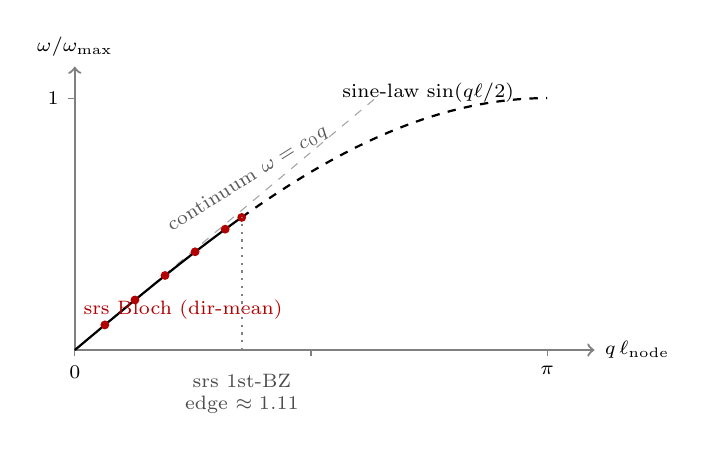
\begin{tikzpicture}[scale=1.0]
    % axes: x = kℓ_node in [0, π] mapped to [0, 6.2832 cm* (2/π)] → use 2 cm per unit-ish
    % choose x-scale so kℓ=π → 6.0 cm; y-scale ω/ω_max in [0,1] → 3.2 cm
    \def\xk{1.9099}  % cm per kℓ unit (π·1.9099 ≈ 6.0)
    \def\yk{3.2}
    \draw[->, thick, gray] (0,0) -- (6.6,0) node[right, font=\scriptsize, black] {$q\,\ell_{\mathrm{node}}$};
    \draw[->, thick, gray] (0,0) -- (0,3.6) node[above, font=\scriptsize, black] {$\omega/\omega_{\max}$};
    % x ticks (π/2 tick label omitted to avoid clashing with the 1st-BZ annotation)
    \draw[gray] (0,0) -- (0,-0.08) node[below, font=\scriptsize, black] {$0$};
    \draw[gray] ({1.5708*\xk},0) -- ({1.5708*\xk},-0.08);
    \draw[gray] ({3.1416*\xk},0) -- ({3.1416*\xk},-0.08) node[below, font=\scriptsize, black] {$\pi$};
    \draw[gray] (0,\yk) -- (-0.08,\yk) node[left, font=\scriptsize, black] {$1$};
    % continuum (dispersionless) reference ω=c₀q ⇒ y = kℓ/π up to y=1 at kℓ=π/... actually
    % small-k slope is 2/π (since ω=c₀q, ω/ω_max = q ℓ /2, so slope in kℓ is 1/2):
    % y = kℓ/2, reaches 1 at kℓ=2. Draw as thin gray dashed straight line.
    \draw[dashed, gray!70] (0,0) -- ({2.0*\xk},{1.0*\yk});
    \node[gray!70!black, font=\scriptsize, rotate=32] at ({1.15*\xk},{0.68*\yk}) {continuum $\omega=c_0q$};
    % TL loaded-line sine-law y=sin(kℓ/2): plot 0..π. Solid within first BZ, dashed beyond.
    % first-BZ edge (srs [100]) at kℓ ≈ 1.1107
    \def\bz{1.1107}
    % solid segment (in first BZ) — overlaps the srs band
    \draw[thick, black] plot[domain=0:1.1107, samples=40] ({\x*\xk},{sin(deg(\x/2))*\yk});
    % dashed continuation past the first BZ (1D-chain band; srs folds here)
    \draw[thick, black, dashed] plot[domain=1.1107:3.1416, samples=60] ({\x*\xk},{sin(deg(\x/2))*\yk});
    \node[black, font=\scriptsize] at ({2.35*\xk},{1.02*\yk}) {sine-law $\sin(q\ell/2)$};
    % srs eigensolve band markers (directional mean), first BZ only — coincide with the solid TL curve
    \foreach \kl/\y in {0.2/0.0999, 0.4/0.1988, 0.6/0.2960, 0.8/0.3901, 1.0/0.4798, 1.11/0.5264} {
        \fill[red!70!black] ({\kl*\xk},{\y*\yk}) circle (1.6pt);
    }
    \node[red!70!black, font=\scriptsize] at ({0.72*\xk},{0.16*\yk}) {srs Bloch (dir-mean)};
    % first-BZ edge marker
    \draw[dotted, thick, gray] ({\bz*\xk},0) -- ({\bz*\xk},{sin(deg(\bz/2))*\yk});
    \node[gray!60!black, font=\scriptsize, align=center] at ({\bz*\xk},-0.55) {srs 1st-BZ\\edge $\approx1.11$};
\end{tikzpicture}
\caption{The bond as a distributed transmission line (Vol.~9 Ch.~3 device-circuit-models \S4; canonical KB \kbleaf{ave-kb/vol4/circuit-theory/ch1-vacuum-circuit-analysis/z0-derivation.md}, \S``The Bond as a Distributed Transmission Line''). \textbf{(a)}~Each K4/srs bond is a lossless TL segment of length $\ell_{\mathrm{node}}$, per-length $\mu_0,\varepsilon_0$ $\Rightarrow$ $Z_0=\sqrt{\mu_0/\varepsilon_0}\approx\SI{376.73}{\ohm}$, delay $\tau=\sqrt{L_{\mathrm{cell}}C_{\mathrm{cell}}}=\ell_{\mathrm{node}}/c_0$ ($L_{\mathrm{cell}}=\mu_0\ell_{\mathrm{node}}$, $C_{\mathrm{cell}}=\varepsilon_0\ell_{\mathrm{node}}$; \kbleaf{src/ave/core/constants.py} \texttt{L\_CELL}, \texttt{C\_CELL}). The \#519 lumped node is the $\omega\tau\ll1$ limit; the lumped and distributed ABCD first diverge at $O(\theta^2)$ ($A_{\mathrm{lump}}-A_{\mathrm{line}}=-\theta^2/2$, $D$-part $+\theta^2/2$). \textbf{(b)}~The periodically-loaded-line Bloch condition $\cos(q\ell)=\mathrm{tr(ABCD)}/2$ gives $\omega(q)=(2c_0/\ell_{\mathrm{node}})|\sin(q\ell_{\mathrm{node}}/2)|$ (solid; the canonical LC-ladder sine-law, \kbleaf{ave-kb/vol4/circuit-theory/ch1-vacuum-circuit-analysis/graded-network-response.md}, clm-gvn4r1). The genuine 24$\times$24 chiral-srs Bloch eigensolve (\kbleaf{src/scripts/vol\_4\_engineering/srs\_bloch\_dispersion.py}) directional-mean (red) coincides with the sine-law within the first Brillouin zone ($q\ell<1.11$; TL/Bloch rel-dev $<2\times10^{-3}$, \kbleaf{research/2026-07-04\_bond-transmission-line\_result.md}). Beyond the srs first-BZ edge the 1D-chain sine-law (dashed) enters the srs folded bands (different Brillouin zone). The srs \emph{rank-2} zone-edge anisotropy (which the scalar 1D TL cannot host) grows to $\sim4.6\times10^{-2}$ at the edge, re-confirming the existing weak-C zone-edge flag (gate \texttt{wejkhvnfb} OPEN). Consistency-class re-expression.}
\label{fig:vol9_circuit_bond_transmission_line}
\end{figure}
